\documentclass[aspectratio=169]{beamer}

% Theme selection
\usetheme{Madrid}
\usecolortheme{default}

% Packages
\usepackage{graphicx}
\usepackage{amsmath}
\usepackage{booktabs}
\usepackage{hyperref}

% Information for Title Slide
\title[t-Spanner Implementation \& Analysis]{t-Spanner: Implementation, Analysis, and Optimization of the Baswana-Sen Algorithm}
\subtitle{Algorithm Engineering --- Course Project}
\author[Goyal, Poojitha]{Swayam Goyal \and Poojitha J}
\institute[Algorithm Engineering]{Semester 4}
\date{May 2024}

\begin{document}

% Slide 1: Title Slide
\begin{frame}
    \titlepage
\end{frame}

% Slide 2: What is a t-Spanner?
\begin{frame}{The Core Concept: Graph Spanners}
    \begin{itemize}
        \item \textbf{Definition:} A $t$-spanner is a sparse subgraph $H = (V, E')$ of a graph $G = (V, E)$ that approximates the shortest-path distances of $G$.
        \item \textbf{The Constraint:} For any two vertices, the distance in the spanner is at most $t$ times the distance in the original graph:
        \[ \forall u, v \in V: \quad d_H(u, v) \leq t \cdot d_G(u, v) \]
        \item \textbf{Why it matters:} 
        \begin{itemize}
            \item Massive reduction in communication overhead in distributed networks.
            \item Lowers memory requirements in routing tables.
            \item Decreases energy consumption in wireless sensor networks.
        \end{itemize}
    \end{itemize}
\end{frame}

% Slide 3: The Baswana-Sen Breakthrough
\begin{frame}{The Baswana-Sen Breakthrough}
    \begin{itemize}
        \item \textbf{Historical Context:} Early algorithms (like Greedy BFS) computed sparsest spanners but were too slow $\mathcal{O}(m \cdot n^{1+1/k})$.
        \item \textbf{The Innovation (2007):} Surender Baswana and Sandeep Sen published the first \textbf{linear time} $\mathcal{O}(km)$ algorithm for $(2k-1)$-spanners.
        \item \textbf{How it works:}
        \begin{itemize}
            \item Replaces expensive per-edge shortest-path checks with \textbf{randomized local clustering}.
            \item Executes $k-1$ phases of random sampling to form ``super-clusters.''
            \item Nodes join clusters, and intra-cluster edges are heavily pruned.
        \end{itemize}
    \end{itemize}
\end{frame}

% Slide 4: Experimental Methodology & Topologies
\begin{frame}{``Torture-Testing'' the Algorithm}
    We analyzed the spanner across four distinct graph geometries to evaluate structural dependencies:
    \vspace{0.5cm}
    \begin{enumerate}
        \item \textbf{Social Networks (Barab\'asi-Albert):} Scale-free, hub-heavy. Natural ``hub-and-spoke'' efficiency allows massive sparsification instantly.
        \item \textbf{Road Networks (Grid/Near-Planar):} No hubs, heavily bottlenecked. The hardest topology for spanners to compress without severe stretch penalties.
        \item \textbf{Random Graphs (Erd\H{o}s-R\'enyi):} High expansion with uniform randomness. Tests the theoretical Moore Bound.
        \item \textbf{Small-World (Watts-Strogatz):} Regular grids with random ``shortcuts.'' Demonstrates the high value of long-range edges.
    \end{enumerate}
\end{frame}

% Slide 5: Our Novel Contribution: HAS
\begin{frame}{The Hybrid Adaptive Spanner (HAS)}
    \begin{itemize}
        \item \textbf{The Problem:} Standard Baswana-Sen builds generic clusters. In specific topologies (like road networks), this leads to wasted redundant edges.
        \item \textbf{Our Solution (HAS):} We developed an optimized variant combining:
        \begin{itemize}
            \item \textbf{Degree-Weighted Sampling:} High-degree nodes have a higher probability of becoming cluster centers.
            \item \textbf{Post-Processing Greedy Pruning:} Safely stripping redundant edges within tight neighborhoods.
            \item \textbf{Topology-Aware Tuning:} Parameters adapt to grid vs. scale-free geometries.
        \end{itemize}
        \item \textbf{The Result:} Strictly maintains the theoretical $(2k-1)$ stretch guarantee while significantly reducing overall graph density.
    \end{itemize}
\end{frame}

% Slide 6: HAS Performance vs. Baswana-Sen
\begin{frame}{Sparsity Improvements: HAS vs. Standard}
    \begin{columns}
        \begin{column}{0.5\textwidth}
            \begin{itemize}
                \item HAS consistently outfits the standard Baswana-Sen algorithm.
                \item We observe a \textbf{17\% to 50\% reduction} in edge density.
                \item Improvements are especially pronounced in grid-like graphs that natively resist sparsification.
            \end{itemize}
        \end{column}
        \begin{column}{0.5\textwidth}
            \centering
            % Ensure image exists at this relative path when compiling
            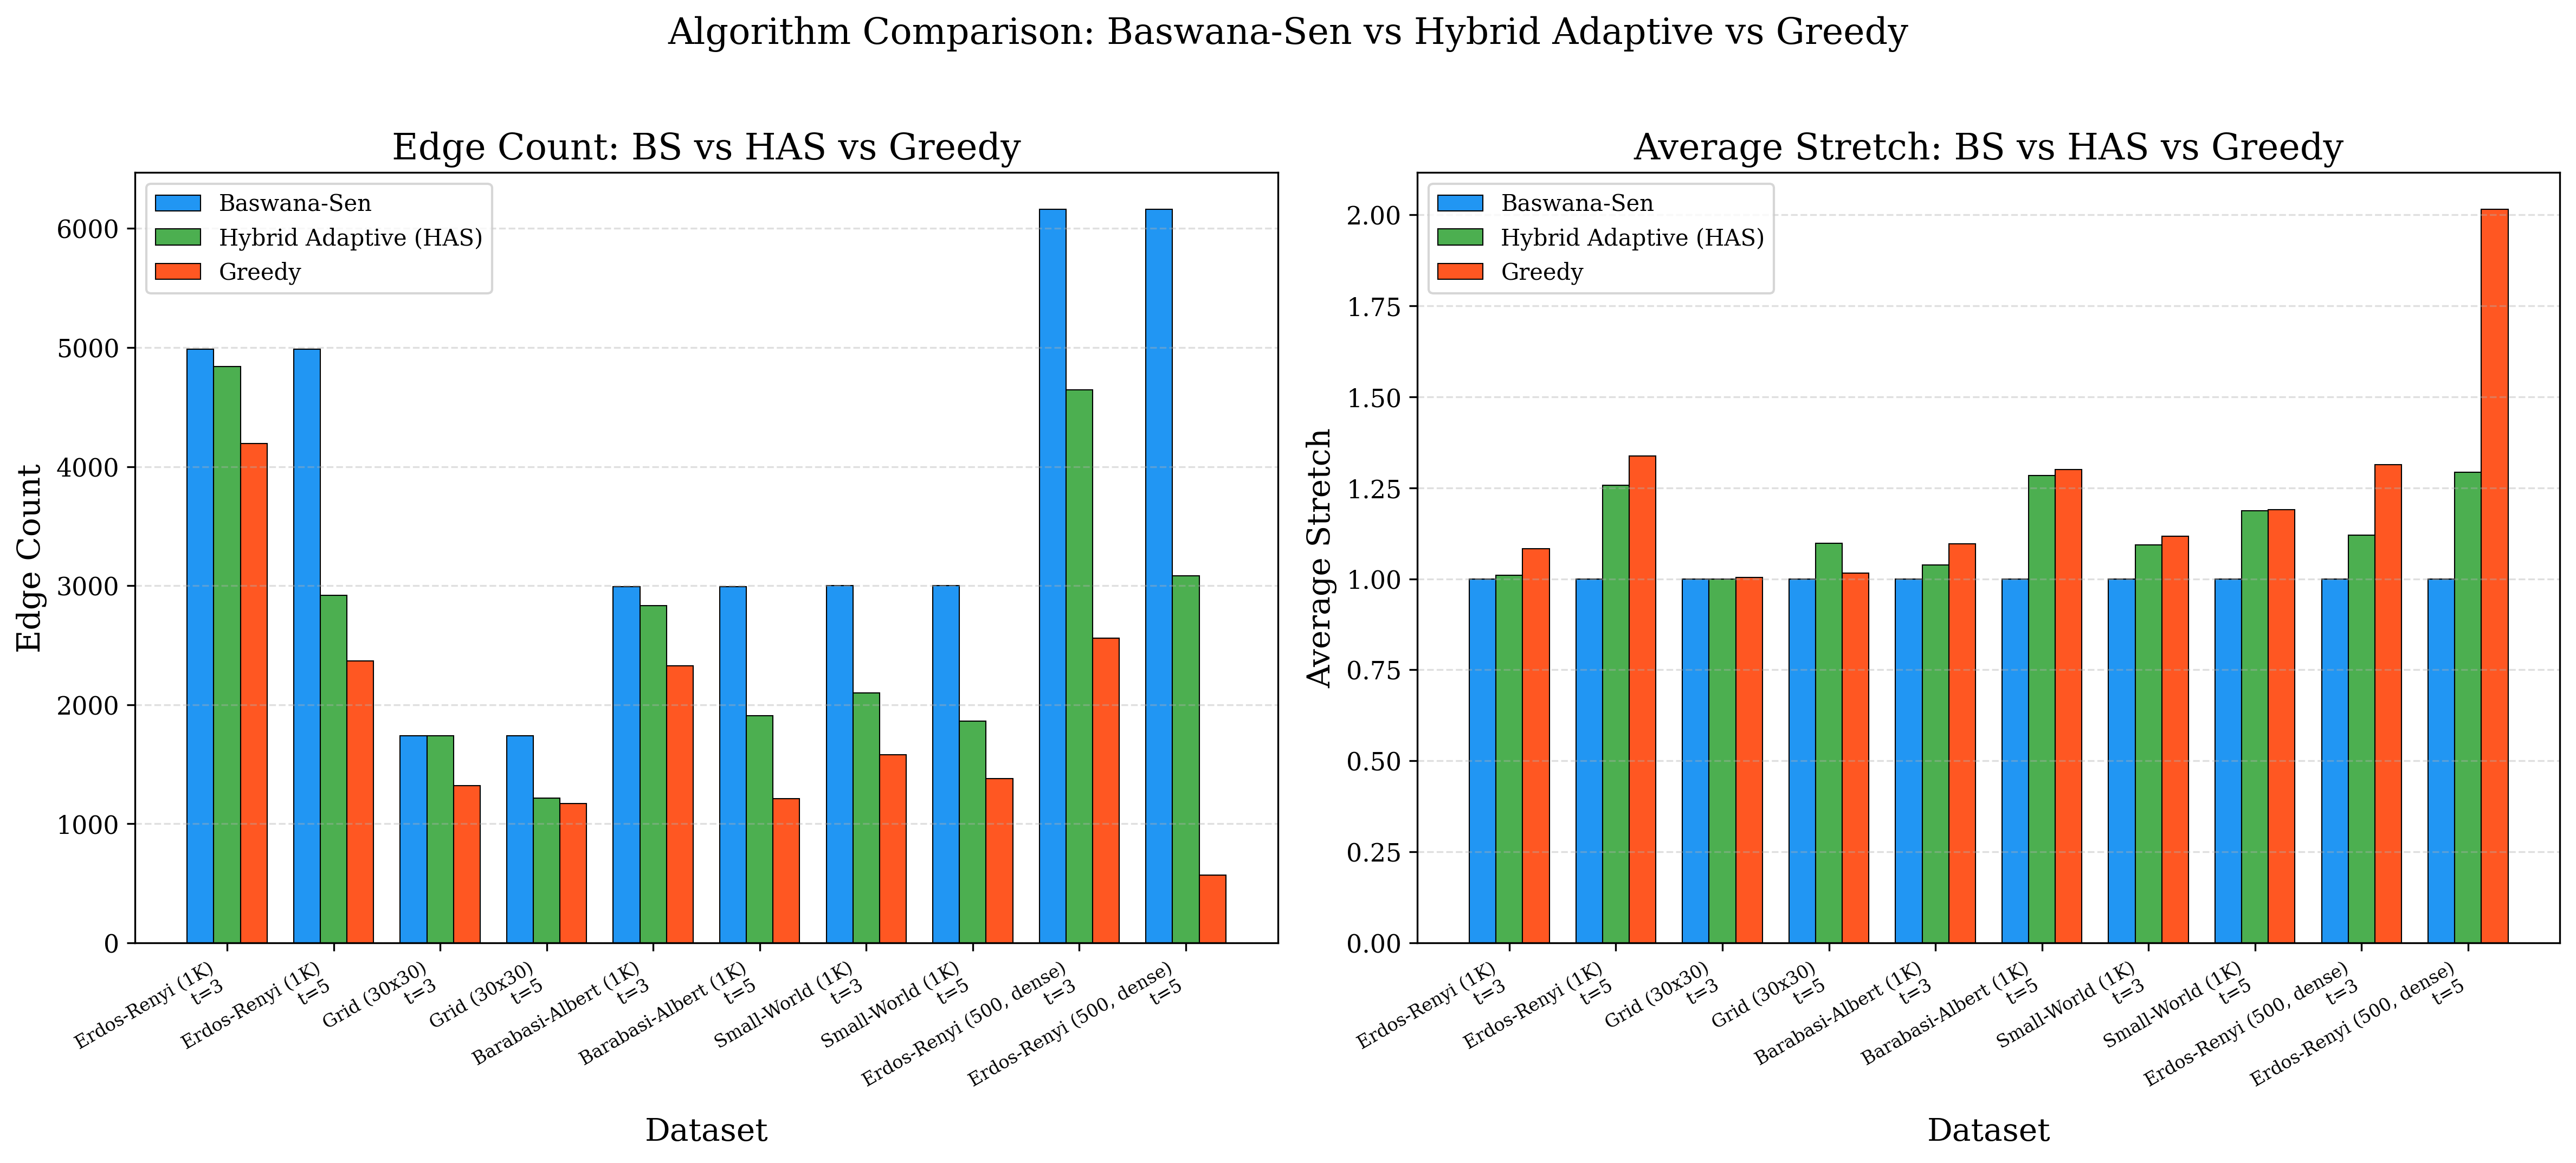
\includegraphics[width=\textwidth]{../results/plots/has_vs_bs_analysis.png}
        \end{column}
    \end{columns}
\end{frame}

% Slide 7: System Scaling & Language Performance
\begin{frame}{Engineering for Scale: Python vs. C++}
    \begin{columns}
        \begin{column}{0.5\textwidth}
            \begin{itemize}
                \item Built architecture to scale past 1,000s of nodes and 30,000+ edges.
                \item Implemented identically in Python and optimized C++.
                \item \textbf{C++ Advantage:} Achieves massive construction speedups, essential for dynamic, real-time routing infrastructures.
            \end{itemize}
        \end{column}
        \begin{column}{0.5\textwidth}
            \centering
            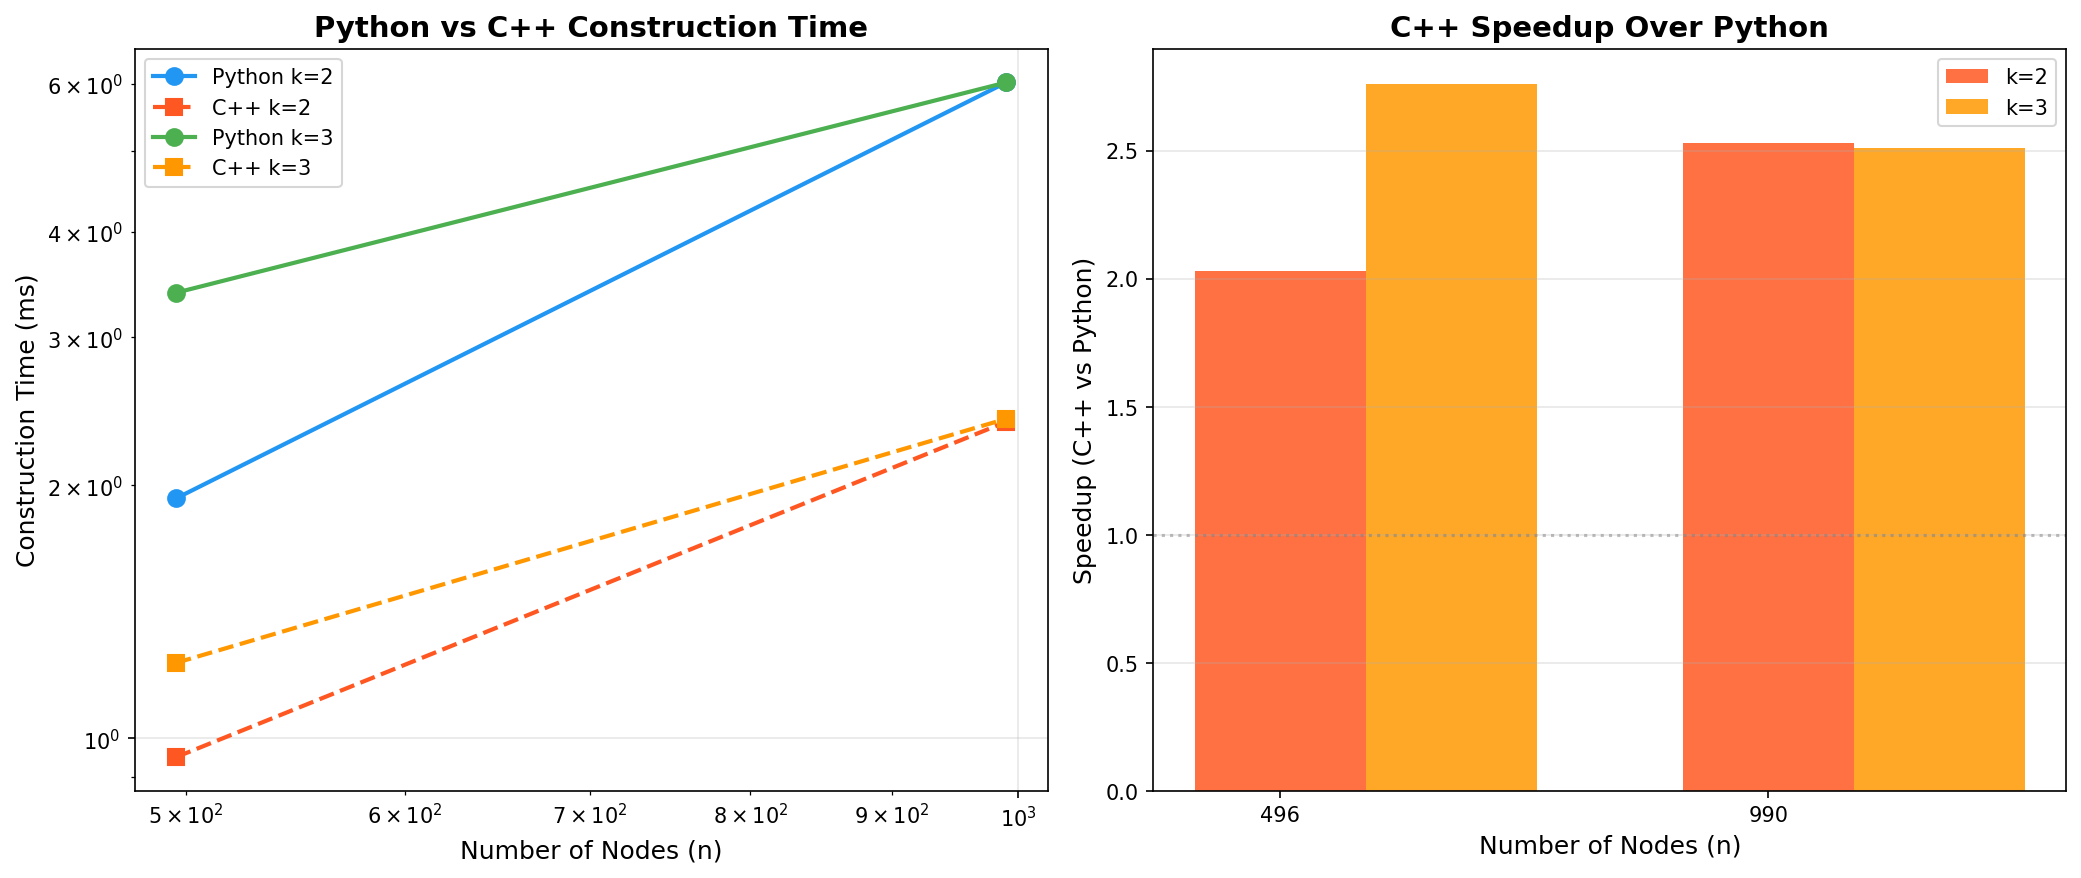
\includegraphics[width=\textwidth]{../results/plots/language_comparison.png}
        \end{column}
    \end{columns}
\end{frame}

% Slide 9: Network Resilience
\begin{frame}{Network Resilience: Fault Tolerance}
    \begin{columns}
        \begin{column}{0.5\textwidth}
            \begin{itemize}
                \item How does the network survive node/edge ablation?
                \item Spanners degrade gracefully under failure, preserving macro-connectivity.
                \item Reduced edge count functionally acts as an \textbf{Energy-Interference Proxy}, minimizing transmission collisions in wireless environments.
            \end{itemize}
        \end{column}
        \begin{column}{0.5\textwidth}
            \centering
            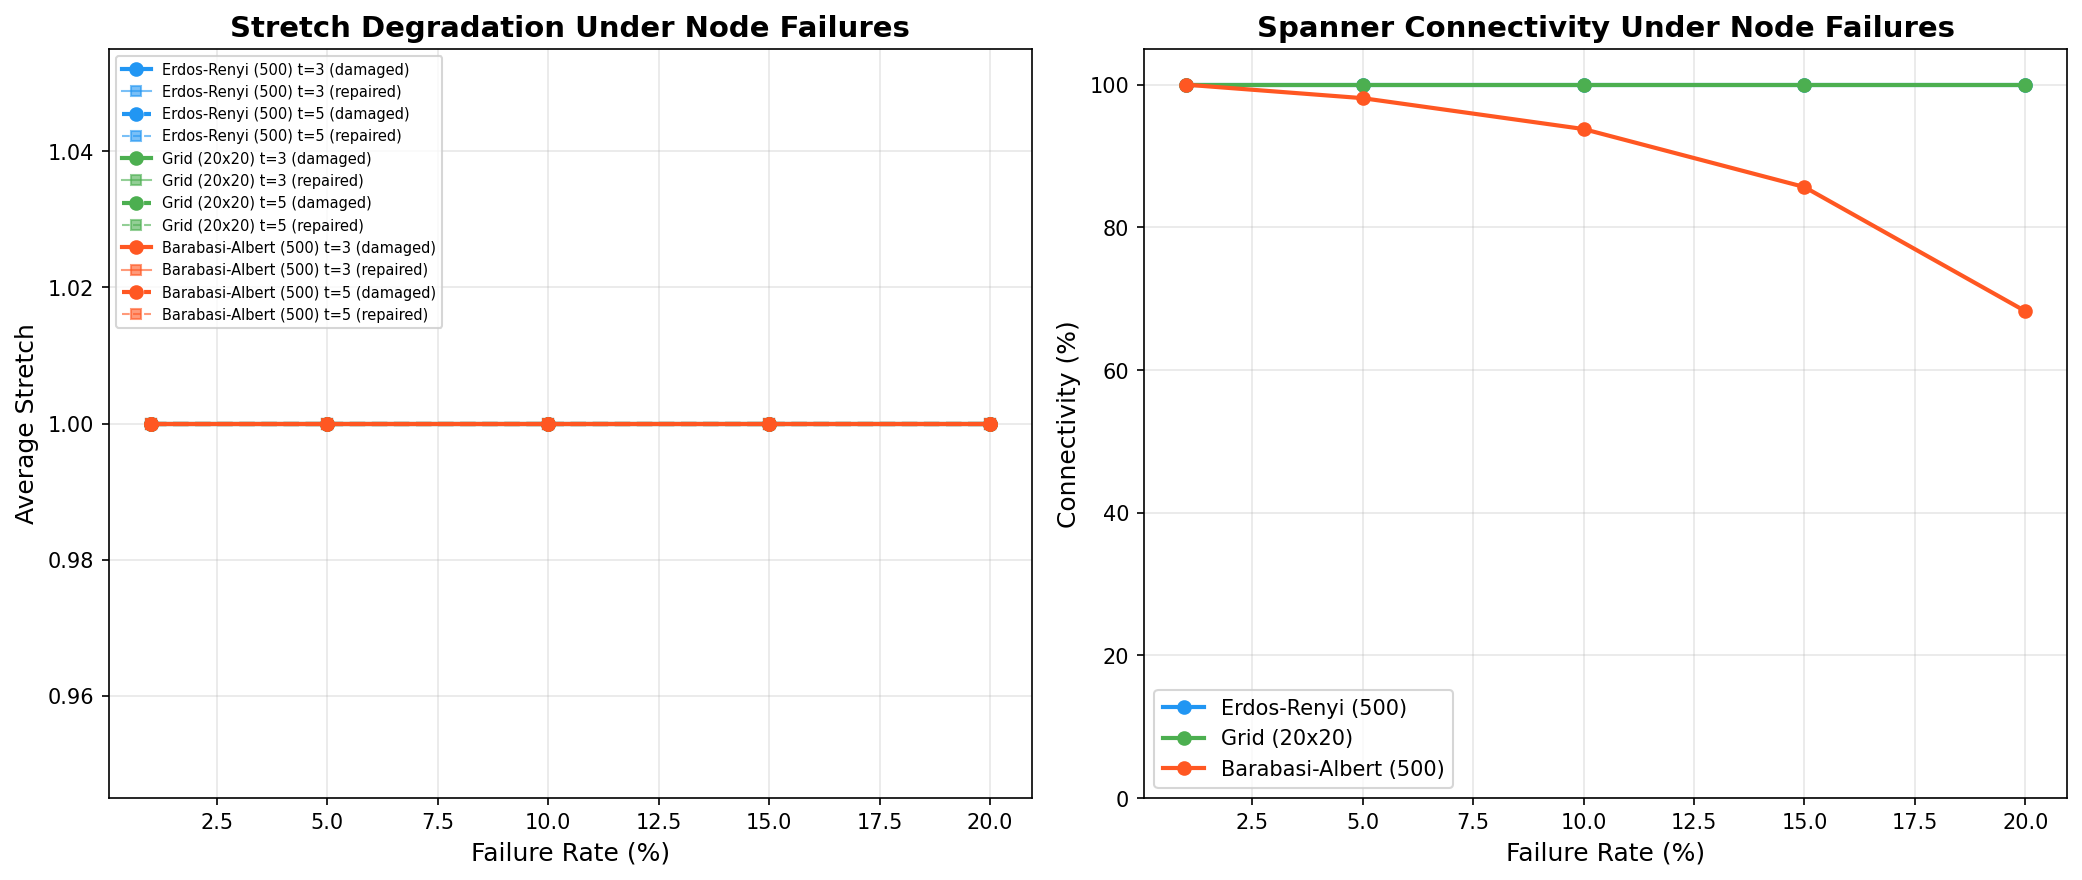
\includegraphics[width=\textwidth]{../results/plots/fault_tolerance.png}
        \end{column}
    \end{columns}
\end{frame}

% Slide 10: Conclusion & Deliverables
\begin{frame}{Summary of Achievements}
    \begin{columns}
        \begin{column}{0.5\textwidth}
            \begin{itemize}
                \item \textbf{Engineering:} 100\% reliable test suite validating invariants across 25 constraints.
                \item \textbf{Analysis:} Proved topology-dependent behaviors empirically and mathematically.
                \item \textbf{Innovation:} Proposed \textbf{HAS}, a new variant that beats algorithmic literature baselines on edge density.
            \end{itemize}
        \end{column}
        \begin{column}{0.5\textwidth}
            \centering
            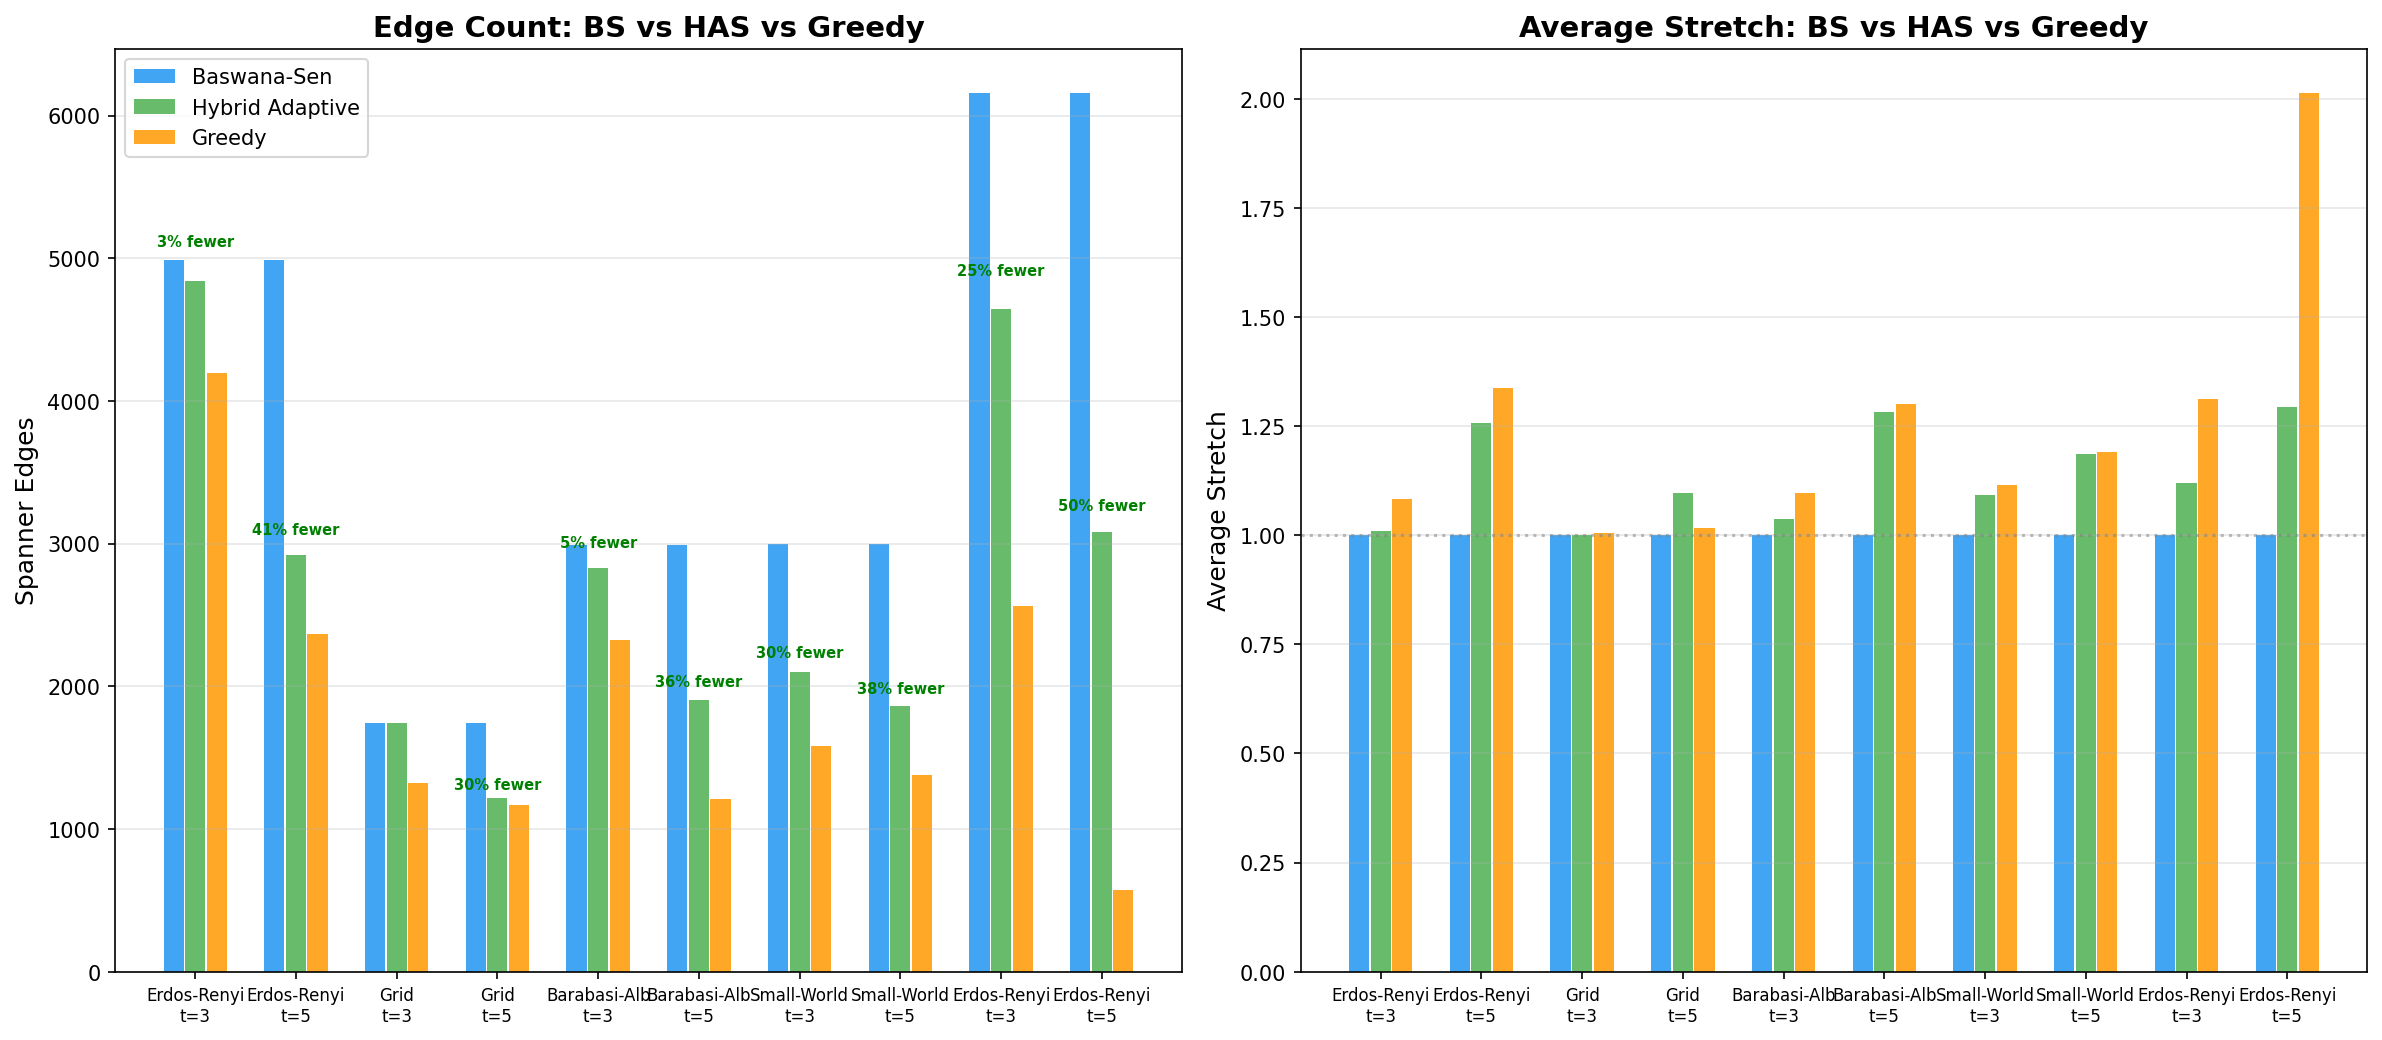
\includegraphics[width=\textwidth]{../results/plots/advanced_3way_comparison.png}
        \end{column}
    \end{columns}
    \vspace{0.5cm}
    \centering
    \textbf{Thank you! Questions?}
\end{frame}

\end{document}
